% ============================================================
%  Proyecto Final de Aprendizaje Automático
%  Escuela Politécnica Superior — Universidad de Alicante
%  Formato: artículo científico (una columna)
% ============================================================

\documentclass[11pt,a4paper]{article}

\usepackage[utf8]{inputenc}
\usepackage[T1]{fontenc}
\usepackage[spanish,es-tabla]{babel}
\usepackage[margin=2.5cm]{geometry}
\usepackage{amsmath}
\usepackage{amssymb}
\usepackage{bm}
\usepackage{graphicx}
% Las imágenes se buscan directamente en la raíz del proyecto de Overleaf.
\graphicspath{{./}}
\usepackage{booktabs}
\usepackage{multirow}
\usepackage{array}
\usepackage{float}
\usepackage{listings}
\usepackage{xcolor}

\lstset{
    language=Python,
    basicstyle=\ttfamily\footnotesize,
    keywordstyle=\color{blue},
    commentstyle=\color{gray},
    stringstyle=\color{red!70!black},
    showstringspaces=false,
    breaklines=true,
    frame=single,
    numbers=left,
    numberstyle=\tiny\color{gray}
}

\usepackage{hyperref}
\hypersetup{
    colorlinks=true,
    linkcolor=blue!70!black,
    citecolor=blue!70!black,
    urlcolor=blue!70!black
}

\usepackage{microtype}


% ============================================================
%  DATOS DEL TRABAJO
% ============================================================

\title{
    \textbf{Análisis de Sesgo Racial y Robustez Adversaria en COMPAS}\\[4pt]
    \large Comparativa de estrategias de equidad para la predicción de reincidencia bajo el marco del Reglamento Europeo de IA
}

\author{
    \textbf{Santiago Álvarez Geanta}\thanks{\texttt{sag82@alu.ua.es}}
    \quad
    \textbf{Taron Sargsyan}\thanks{\texttt{ts73@alu.ua.es}}
    \quad
    \textbf{Joaquín Sigüenza Chilar}\thanks{\texttt{jsc114@alu.ua.es}}
    \\[4pt]
    \small Grado en Ingeniería en Inteligencia Artificial
    --- Escuela Politécnica Superior, Universidad de Alicante\\
    \small Aprendizaje Avanzado --- Curso 2025/2026
}

\date{}

% ============================================================

\begin{document}

\maketitle
\thispagestyle{empty}

% Abstract

\begin{abstract}
\noindent El sistema COMPAS, empleado en tribunales de Estados Unidos para estimar la reincidencia de acusados, fue señalado en 2016 por ProPublica como discriminatorio contra la población afroamericana, con una tasa de falsos positivos que duplicaba la del grupo caucásico. Este trabajo replica y amplía dicho análisis sobre el \textit{dataset} \textit{COMPAS-two-years} (aprox.\ 6\,000 instancias tras el filtrado de ProPublica, restringido a los grupos afroamericano y caucásico) abordando dos problemáticas no triviales: la \textit{equidad algorítmica} y la \textit{robustez adversaria}. Se entrena un modelo \textit{baseline} de Regresión Logística que se compara, mediante el optimizador de umbral de \texttt{fairlearn}, frente a tres restricciones de equidad: paridad demográfica, paridad de tasa de falsos positivos (FPR) y \textit{equalized odds}. La explicabilidad se aborda con valores SHAP exactos sobre el modelo lineal y la robustez con el método de Gradiente Rápido (FGM, $\varepsilon{=}0{,}1$) del \textit{Adversarial Robustness Toolbox}. Los resultados confirman cuantitativamente el sesgo documentado por ProPublica en el \textit{baseline} y revelan un \textit{trade-off} explícito entre precisión y equidad: la paridad de FPR reduce de manera sustancial la disparidad racial a cambio de una pérdida moderada de \textit{accuracy} global, mientras que el ataque adversario provoca una caída notable de precisión, incompatible con los requisitos de robustez exigidos a los sistemas de alto riesgo por el Reglamento (UE) 2024/1689.
\end{abstract}

\smallskip
\noindent\textbf{Palabras clave:} aprendizaje automático, equidad algorítmica, COMPAS, sesgo racial, robustez adversaria, EU~AI~Act, explicabilidad (SHAP).

\tableofcontents
\newpage


% ============================================================
\section{Introducción}
% ============================================================

Los sistemas de decisión automatizada se han incorporado a ámbitos donde un error o un sesgo no es un fallo técnico aislado, sino una vulneración de derechos fundamentales. COMPAS (\textit{Correctional Offender Management Profiling for Alternative Sanctions}), desarrollado por Northpointe~\cite{northpointe2015practitioner}, asigna a cada acusado un \textit{decile score} de riesgo de reincidencia que jueces de varios estados de Estados Unidos utilizan como factor en decisiones sobre prisión preventiva, libertad condicional o sentencia. Como demostró la investigación de ProPublica en 2016~\cite{angwin2016machine, propublica_compas_2016}, este sistema asignaba puntuaciones de alto riesgo a personas afroamericanas con una frecuencia significativamente superior a la observada empíricamente: la tasa de falsos positivos para acusados afroamericanos prácticamente duplicaba la del grupo caucásico. El caso \textit{State v.\ Loomis} (2016) en Wisconsin extendió el debate al plano constitucional, al permitir el uso del sistema en sentencia pese a su opacidad.

Las implicaciones del fenómeno trascienden lo técnico. En el plano ético, automatizar una predicción anclada en un registro histórico sesgado sobre poblaciones racializadas reproduce y amplifica una discriminación estructural~\cite{barocas2019fairness}. En el plano jurídico, el Reglamento (UE) 2024/1689 (\textit{EU AI Act})~\cite{eu_ai_act_2024} clasifica los sistemas de IA destinados a la \emph{administración de justicia y procesos democráticos} (Anexo~III, punto~8) como de \textbf{alto riesgo}, lo que impone obligaciones estrictas de gestión de riesgo (Art.~9), calidad de los datos (Art.~10), transparencia (Art.~13), supervisión humana (Art.~14) y robustez (Art.~15). El Reglamento General de Protección de Datos~\cite{gdpr2016} limita además las decisiones automatizadas con efectos jurídicos significativos sobre las personas (Art.~22) y refuerza la protección de categorías especiales de datos como las relativas a infracciones penales (Art.~10).

Sobre este marco, el presente trabajo aborda dos problemáticas avanzadas de aprendizaje automático justificadas por el dominio: \emph{(i)}~la \textbf{equidad algorítmica}, comparando cuatro criterios de optimización (precisión global, paridad demográfica, paridad de FPR y \textit{equalized odds}) implementados como post-procesamiento sobre un modelo \textit{baseline} de Regresión Logística~\cite{hardt2016equality, bird2020fairlearn}; y \emph{(ii)}~la \textbf{robustez adversaria}, mediante un ataque de gradiente rápido (FGM) que simula manipulaciones realistas de las variables de entrada~\cite{goodfellow2015explaining, nicolae2018art}. La explicabilidad por valores SHAP~\cite{lundberg2017unified} complementa el análisis identificando la \textit{proxy discrimination} que ejercen variables aparentemente neutras como el número de condenas previas o la edad.

El resto del artículo se organiza como sigue.
La Sección~\ref{sec:related} revisa el trabajo relacionado.
La Sección~\ref{sec:datos} describe el \textit{dataset} y el análisis exploratorio.
La Sección~\ref{sec:metodologia} detalla la metodología.
La Sección~\ref{sec:resultados} presenta los resultados experimentales.
La Sección~\ref{sec:discusion} discute las implicaciones técnicas, éticas y legales.
La Sección~\ref{sec:conclusiones} concluye el trabajo.


% ============================================================
\section{Trabajo Relacionado}
\label{sec:related}
% ============================================================

\subsection{El caso COMPAS y la auditoría algorítmica de sistemas judiciales}

La denuncia de ProPublica~\cite{angwin2016machine} popularizó la noción de \textit{algorithmic bias} y reveló una disparidad sistemática de falsos positivos entre acusados afroamericanos y caucásicos en COMPAS. La réplica de Northpointe~\cite{dieterich2016compas} sostuvo que el sistema era equitativo bajo \textit{predictive parity} (calibración por grupo). Chouldechova~\cite{chouldechova2017fair} formalizó la incompatibilidad: cuando la prevalencia del evento difiere entre grupos, la paridad predictiva y la paridad de errores no pueden satisfacerse simultáneamente, conclusión equivalente al teorema de imposibilidad de Kleinberg, Mullainathan y Raghavan~\cite{kleinberg2017inherent}. Dressel y Farid~\cite{dressel2018accuracy} mostraron, además, que la precisión de COMPAS es comparable a la de personas no expertas con apenas dos variables (edad y condenas previas), lo que cuestiona la utilidad marginal de un sistema opaco y caro.

\subsection{Técnicas de equidad algorítmica}

La literatura distingue tres familias de intervenciones: \emph{pre-procesamiento} (transformación de los datos previa al entrenamiento)~\cite{kamiran2012data, calmon2017optimized}, \emph{in-processing} (restricciones de equidad incorporadas a la función objetivo)~\cite{zafar2017fairness, agarwal2018reductions} y \emph{post-procesamiento} (ajuste de los umbrales de decisión a posteriori)~\cite{hardt2016equality, pleiss2017fairness}. Las definiciones formales más utilizadas son la \textit{demographic parity}~\cite{dwork2012fairness}, la \textit{equalized odds} y la \textit{equal opportunity}~\cite{hardt2016equality}. Las bibliotecas \texttt{fairlearn}~\cite{bird2020fairlearn} y \texttt{AIF360}~\cite{bellamy2018aif360} consolidan implementaciones reproducibles de estas técnicas. Este trabajo se apoya en post-procesamiento (\texttt{ThresholdOptimizer}) por su bajo coste computacional y porque permite reutilizar un \textit{baseline} ya entrenado sin alterar su representación interna.

\subsection{Explicabilidad y robustez adversaria}

La explicabilidad mediante atribución de variables se ha consolidado con SHAP (\textit{Shapley Additive Explanations})~\cite{lundberg2017unified}, que unifica métodos previos como LIME~\cite{ribeiro2016lime}. Para modelos lineales, \texttt{shap.LinearExplainer} ofrece valores SHAP exactos, lo que evita el ruido de las aproximaciones Monte Carlo y resulta especialmente relevante en auditorías de equidad. En paralelo, el descubrimiento de los ejemplos adversarios~\cite{szegedy2014intriguing, goodfellow2015explaining} expuso una vulnerabilidad estructural de los clasificadores: pequeñas perturbaciones $\delta$ con $\|\delta\|_\infty \leq \varepsilon$ pueden alterar la predicción. El \textit{Adversarial Robustness Toolbox} (ART)~\cite{nicolae2018art} estandariza estos ataques y defensas; su evaluación es una práctica recomendable para cualquier sistema clasificado como de alto riesgo bajo el EU~AI~Act~\cite{eu_ai_act_2024}.


% ============================================================
\section{Descripción del Problema y los Datos}
\label{sec:datos}
% ============================================================

\subsection{Definición formal de la tarea}

Sea $\bm{x}\in\mathcal{X}\subseteq\mathbb{R}^d$ el vector de \textit{features} de un acusado (edad, género, recuento de condenas previas, gravedad del cargo actual, etc.) e $y\in\mathcal{Y}=\{0,1\}$ la variable objetivo \texttt{two\_year\_recid} ($y{=}1$ si el individuo reincide en los dos años posteriores). Sea $a\in\mathcal{A}=\{\text{African-American},\text{Caucasian}\}$ el atributo sensible \texttt{race}, no utilizado como \textit{feature} de entrada. La tarea es un problema de \textbf{clasificación binaria supervisada}: aprender $f_\theta\colon\mathcal{X}\to[0,1]$ que minimice el riesgo esperado
\begin{equation}
    \theta^\star = \arg\min_\theta \;\mathbb{E}_{(\bm{x},y)\sim\mathcal{D}}\bigl[\,\ell\bigl(f_\theta(\bm{x}),y\bigr)\bigr],
    \label{eq:erm}
\end{equation}
con $\ell$ la pérdida de entropía cruzada binaria, estimada empíricamente sobre el conjunto de entrenamiento $\mathcal{D}_{\text{train}}=\{(\bm{x}_i,y_i)\}_{i=1}^{N}$. Adicionalmente, denotamos $\hat{Y}=\mathbb{1}\{f_\theta(\bm{x})\geq\tau\}$ con $\tau$ el umbral de decisión (eventualmente \emph{dependiente del grupo} $a$, según la Sección~\ref{sec:metod_fairness}).

\subsection{Dataset}

El \textit{dataset} \textit{COMPAS Recidivism — Two-Year} fue recopilado y publicado por ProPublica~\cite{propublica_compas_2016} a partir de registros del condado de Broward (Florida). Tras aplicar el filtrado original de ProPublica (Sección~\ref{sec:preproc}) y restringir el análisis a los grupos afroamericano y caucásico, se obtienen las características recogidas en la Tabla~\ref{tab:dataset}. Los individuos representados son acusados detenidos en Broward (FL, EE.UU.) entre 2013 y 2014; los datos fueron recogidos por Northpointe en el contexto de una herramienta comercial, por lo que el muestreo refleja la práctica policial y judicial local y arrastra sesgos de selección documentados (mayor presencia policial en barrios racializados, criminalización diferencial de delitos menores). La variable \texttt{race} se utiliza únicamente como atributo sensible para la evaluación y mitigación, nunca como predictor.

\begin{table}[H]
\centering
\caption{Características del \textit{dataset} \textit{COMPAS-two-years} tras el filtrado de ProPublica.}
\label{tab:dataset}
\small
\begin{tabular}{@{}ll@{}}
\toprule
\textbf{Característica} & \textbf{Valor} \\
\midrule
Fuente / enlace           & ProPublica (GitHub: \texttt{propublica/compas-analysis}) \\
Número de instancias      & $\approx 6\,000$ (tras filtrado y selección de razas) \\
Número de \textit{features} (modelado) & 8 (5 numéricas, 3 categóricas)\\
Variable objetivo         & \texttt{two\_year\_recid} (binaria) \\
Atributo sensible         & \texttt{race} $\in\{$African-American, Caucasian$\}$ \\
Distribución de clases    & $\approx 55\,\%$ no reincide $/\;45\,\%$ reincide \\
Valores ausentes          & Sí $\to$ imputación: mediana (num.), moda (cat.) \\
Licencia                  & Dominio público (datos administrativos liberados por FOIA) \\
\bottomrule
\end{tabular}
\end{table}

\subsection{Análisis exploratorio (EDA)}

El EDA persigue tres objetivos: \emph{(i)}~verificar el desbalanceo de clases, \emph{(ii)}~contrastar la prevalencia real de reincidencia por grupo racial, y \emph{(iii)}~exponer el sesgo de la puntuación COMPAS original (\texttt{decile\_score}). La distribución por raza está moderadamente desequilibrada (mayor número de acusados afroamericanos, consecuencia del sesgo de selección antes mencionado). La tasa real de reincidencia (\texttt{two\_year\_recid}) difiere entre grupos --- aproximadamente 52\,\% para acusados afroamericanos frente a 39\,\% para caucásicos --- diferencia que la literatura atribuye a desigualdades estructurales previas, no a una propensión criminal diferencial~\cite{barocas2019fairness}. Sin embargo, la distribución del \texttt{decile\_score} es la prueba directa del sesgo del sistema operativo: los acusados afroamericanos concentran su distribución hacia las puntuaciones altas (8--10) mientras que los caucásicos se concentran en las bajas (1--3), con una asimetría que excede lo justificable por la diferencia de prevalencia. Estas observaciones motivan tratar la equidad como un eje analítico de primer orden, no como un control secundario.

\begin{figure}[H]
\centering
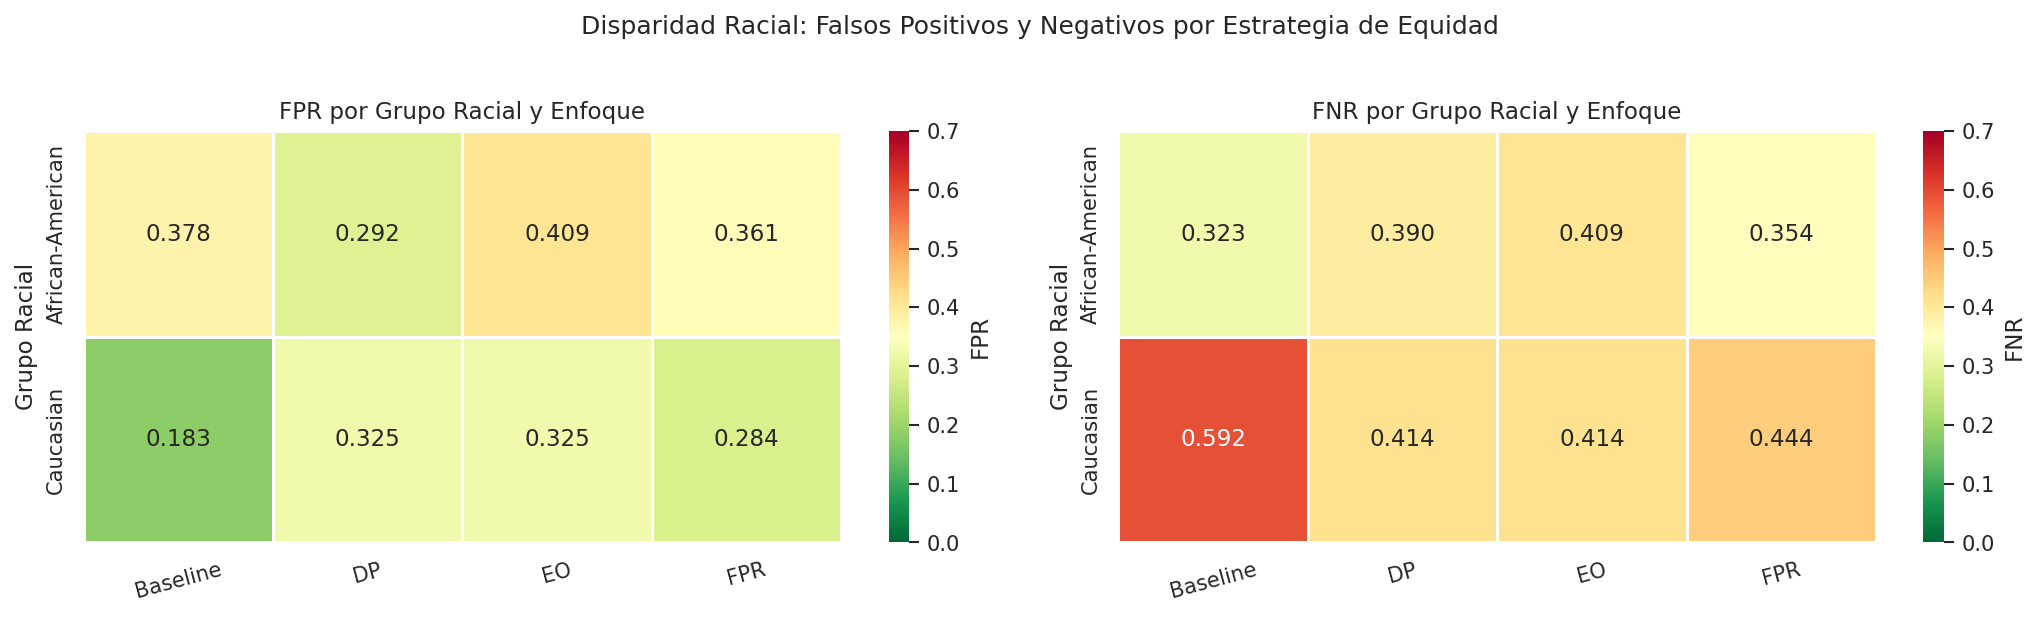
\includegraphics[width=0.85\textwidth]{./figures/group_metrics_heatmap}
\caption{Métricas por grupo racial (\textit{accuracy}, precisión, \textit{recall}, F1, FPR, FNR) para el modelo \textit{baseline} y las tres intervenciones de equidad evaluadas. La fila del \textit{baseline} evidencia la disparidad de FPR (mayor en African-American) y de FNR (mayor en Caucasian) consistente con el resultado de ProPublica.}
\label{fig:eda}
\end{figure}

\subsection{Problemáticas identificadas}

A partir del análisis del \textit{dataset} y del contexto de uso del sistema, se identifican dos problemáticas que el modelo debe abordar de forma explícita:

\begin{itemize}
    \item \textbf{Problemática 1 --- Equidad algorítmica (sesgo racial):} el sistema toma decisiones sobre personas en un dominio (la administración de justicia) clasificado como de \emph{alto riesgo} por el EU~AI~Act. El \textit{dataset} contiene un atributo sensible (\texttt{race}) cuya distribución condiciona claramente la salida del modelo a través de \textit{proxies} (condenas previas, edad), y la evidencia empírica documenta un sesgo histórico cuantificable. No tratar la equidad equivale a reproducirla y, jurídicamente, a incumplir el Art.~10 del EU~AI~Act.
    \item \textbf{Problemática 2 --- Robustez adversaria:} un sistema judicial automatizado opera en un entorno con incentivos para la manipulación: un acusado o su entorno pueden modificar variables declaradas u observables (p.\ ej.\ información sobre antecedentes, gravedad del cargo) para inducir una predicción de bajo riesgo. El Art.~15 del EU~AI~Act exige expresamente robustez frente a errores y ataques. Evaluar esta vulnerabilidad mediante ejemplos adversarios es, por tanto, un requisito de cumplimiento, no un ejercicio académico.
\end{itemize}


% ============================================================
\section{Metodología}
\label{sec:metodologia}
% ============================================================

\subsection{Preprocesamiento}
\label{sec:preproc}

Se aplican los filtros canónicos de ProPublica~\cite{propublica_compas_2016}: se descartan los registros con $|\,$\texttt{days\_b\_screening\_arrest}$\,|>30$, los marcados con \texttt{is\_recid}~$=-1$, los cargos de orden judicial (\texttt{c\_charge\_degree}~$=$~`O') y las puntuaciones inválidas. Posteriormente se restringe el análisis a los acusados de raza afroamericana y caucásica para reproducir el contraste binario del estudio original.

Tras el filtrado se construye el conjunto de \textit{features} de modelado (variables numéricas: \texttt{age}, \texttt{priors\_count}, \texttt{juv\_fel\_count}, \texttt{juv\_misd\_count}, \texttt{juv\_other\_count}; variables categóricas: \texttt{sex}, \texttt{age\_cat}, \texttt{c\_charge\_degree}). Se excluye \texttt{c\_charge\_desc} (alta cardinalidad sin agrupación semántica) y \texttt{decile\_score} (es la propia salida del sistema COMPAS, no una \textit{feature} predictiva genuina). La división \emph{estratificada} \textit{train/test} se realiza con \texttt{test\_size}$=0{,}2$ y \texttt{random\_state}$=80$, manteniendo la prevalencia del objetivo en ambos conjuntos. Críticamente, el \texttt{ColumnTransformer} (imputación por mediana + \texttt{StandardScaler} para numéricas; imputación por moda + \texttt{OneHotEncoder} con \texttt{handle\_unknown=`ignore'} para categóricas) se ajusta \emph{exclusivamente} sobre el conjunto de entrenamiento, dentro de un \texttt{sklearn.Pipeline}, para garantizar la ausencia de \textit{data leakage}.

\subsection{Modelo \textit{baseline}}

El modelo \textit{baseline} es una \textbf{Regresión Logística} con regularización $\ell_2$, optimizada con L-BFGS, \texttt{max\_iter}$=1000$ y \texttt{random\_state}$=80$. La elección se justifica por tres motivos: \emph{(i)}~es el modelo de referencia estándar en la literatura de \textit{algorithmic fairness} sobre COMPAS~\cite{angwin2016machine, hardt2016equality, chouldechova2017fair}, lo que facilita la comparación; \emph{(ii)}~permite calcular valores SHAP \emph{exactos} mediante \texttt{shap.LinearExplainer}, esencial para una auditoría de sesgo rigurosa; y \emph{(iii)}~produce probabilidades calibradas de manera nativa (\texttt{predict\_proba}), requisito de \texttt{ThresholdOptimizer}. Modelos no lineales (Random Forest, GBM, SVM-RBF) ofrecerían potencialmente más precisión, pero a costa de aproximar SHAP por Monte Carlo y dificultar la auditoría, lo que contradice los objetivos del trabajo y las exigencias de explicabilidad del EU~AI~Act (Art.~13).

\subsection{Tratamiento de la problemática 1: equidad algorítmica}
\label{sec:metod_fairness}

Se utiliza una intervención de \emph{post-procesamiento}, \texttt{ThresholdOptimizer} de \texttt{fairlearn}~\cite{hardt2016equality, bird2020fairlearn}, que ajusta umbrales de decisión $\tau_a$ específicos por grupo $a\in\mathcal{A}$ sobre el modelo \textit{baseline} ya entrenado. Formalmente, dada la función score $f_\theta(\bm{x})$, se busca una regla de decisión (posiblemente aleatorizada) $\hat{Y}=h(f_\theta(\bm{x}),a)$ que maximice la precisión sujeta a una restricción de equidad $\mathcal{C}$:
\begin{equation}
    \max_{h\in\mathcal{H}}\;\mathbb{E}\bigl[\mathbb{1}\{\hat{Y}=Y\}\bigr]
    \quad\text{s.\,a.}\quad
    \mathcal{C}(h,A)\le\varepsilon.
    \label{eq:thoptim}
\end{equation}
Se evalúan tres instancias de $\mathcal{C}$ (más el \textit{baseline} sin restricción):
\begin{align}
    \text{Demographic Parity (DP):}\quad &
    \bigl|\,P(\hat{Y}{=}1\mid A{=}a)-P(\hat{Y}{=}1\mid A{=}b)\bigr| \le \varepsilon,
    \label{eq:dp}\\[2pt]
    \text{FPR Parity:}\quad &
    \bigl|\,P(\hat{Y}{=}1\mid Y{=}0, A{=}a)-P(\hat{Y}{=}1\mid Y{=}0, A{=}b)\bigr| \le \varepsilon,
    \label{eq:fpr}\\[2pt]
    \text{Equalized Odds (EO):}\quad &
    \bigl|\,P(\hat{Y}{=}1\mid Y{=}y, A{=}a)-P(\hat{Y}{=}1\mid Y{=}y, A{=}b)\bigr| \le \varepsilon, \ \forall y.
    \label{eq:eo}
\end{align}
Esta elección está motivada empíricamente: en el dominio judicial, un falso positivo (clasificar como reincidente a quien no lo será) tiene un coste social mucho mayor que un falso negativo (privación injusta de libertad versus reincidencia no anticipada), por lo que la \emph{paridad de FPR} es la métrica central de la auditoría, alineada con la denuncia original de ProPublica~\cite{angwin2016machine}. La paridad demográfica se incluye como referencia conceptual, aunque su limitación es conocida~\cite{dwork2012fairness}: puede satisfacerse trivialmente penalizando a uno de los grupos. La \textit{equalized odds} ofrece un compromiso intermedio.

\subsection{Tratamiento de la problemática 2: robustez adversaria}

La robustez se evalúa con un ataque de evasión de gradiente rápido (\textit{Fast Gradient Method}, FGM)~\cite{goodfellow2015explaining} implementado en \texttt{Adversarial Robustness Toolbox} (ART)~\cite{nicolae2018art}. Dado un ejemplo $\bm{x}$ con etiqueta $y$, FGM genera la perturbación
\begin{equation}
    \bm{x}_{\text{adv}} = \bm{x} + \varepsilon\,\operatorname{sign}\!\bigl(\nabla_{\bm{x}}\,\mathcal{L}(f_\theta(\bm{x}),y)\bigr),
    \label{eq:fgm}
\end{equation}
con $\varepsilon=0{,}1$ sobre el espacio ya escalado por \texttt{StandardScaler}. Sobre el \textit{dataset} adversario $\mathcal{D}_{\text{adv}}=\{(\bm{x}_{i,\text{adv}},y_i)\}$ se mide la \textit{accuracy} adversaria y se compara con la limpia; la diferencia $\Delta_{\text{robustness}}$ cuantifica la vulnerabilidad. La elección del FGM se justifica por su carácter de cota inferior de un atacante real (es un ataque de un solo paso, computacionalmente barato): si el modelo cae frente a FGM, caerá frente a ataques iterativos más sofisticados como PGD~\cite{madry2018towards}.

\subsection{Protocolo de evaluación}

La evaluación se descompone en dos niveles. Para \textbf{generalización}, se aplica \emph{validación cruzada estratificada de 5 \textit{folds}} sobre el conjunto de entrenamiento (\texttt{StratifiedKFold}, \texttt{random\_state}$=80$) reportando media~$\pm$~desv.\ típica de \textit{accuracy}, F1, AUC-ROC, precisión y \textit{recall}. La estratificación es necesaria por el desbalanceo y la AUC-ROC es la métrica primaria al ser robusta al desbalanceo. Para \textbf{equidad}, sobre el conjunto de test (intocable hasta la evaluación final) se calculan las métricas por grupo (\texttt{accuracy}, FPR, FNR, F1) mediante \texttt{MetricFrame}, junto con los escalares de disparidad: \emph{demographic parity difference} (DPD), \emph{equalized odds difference} (EOD) y la diferencia de FPR entre grupos. La interpretación es directa: valores próximos a $0$ indican equidad, valores próximos a $1$ indican máxima disparidad.


% ============================================================
\section{Experimentos y Resultados}
\label{sec:resultados}
% ============================================================

\subsection{Configuración experimental}

Todos los experimentos se ejecutan con Python~3.13 y semilla fija \texttt{SEED}$=80$ en todos los procesos estocásticos (división \textit{train/test}, optimizador L-BFGS, validación cruzada y ataque adversario). Las versiones principales son: \texttt{scikit-learn}~1.8, \texttt{fairlearn}~0.13, \texttt{shap}~0.51, \texttt{adversarial-robustness-toolbox}~1.20.1, \texttt{pandas}~3.0.2, \texttt{numpy}~2.4.4. El código fuente y los \textit{notebooks} se encuentran en el repositorio público del proyecto (Anexo~B). El siguiente fragmento ilustra la configuración mínima de reproducibilidad:

\begin{lstlisting}[caption={Semilla aleatoria y entorno principal.}]
import numpy as np
SEED = 80
np.random.seed(SEED)
# sklearn.__version__       == '1.8.0'
# fairlearn.__version__     == '0.13.0'
# shap.__version__          == '0.51.0'
# art.__version__           == '1.20.1'
\end{lstlisting}

\subsection{Resultados comparativos}

La Tabla~\ref{tab:resultados} compara el rendimiento del \textit{baseline} con las tres intervenciones de equidad. Las métricas de generalización (AUC-ROC y F1) corresponden a validación cruzada de 5 \textit{folds} sobre el conjunto de entrenamiento; las métricas de equidad se reportan sobre el conjunto de test. La columna \textit{FPR diff.} ($|\text{FPR}_{\text{AA}}-\text{FPR}_{\text{Cau}}|$) es la métrica específica más relevante en este dominio.

\begin{table}[H]
\centering
\caption{Comparativa de resultados. AUC-ROC y F1: media~$\pm$~desv.\ estándar sobre validación cruzada 5~\textit{folds}. Accuracy, DPD, EOD y FPR diff.\ sobre test (para las métricas de equidad, el intervalo es $[0,1]$ y menor es mejor).}
\label{tab:resultados}
\small
\begin{tabular}{@{}lcccccc@{}}
\toprule
\textbf{Modelo / Configuración} & \textbf{Accuracy} & \textbf{AUC-ROC} & \textbf{F1} & \textbf{DPD} & \textbf{EOD} & \textbf{FPR diff.}\\
\midrule
\textit{Baseline} (Reg. Log.)   & $0{,}6648$ & $0{,}7312 \pm 0{,}0210$ & $0{,}6393 \pm 0{,}0276$ & $0{,}2899$ & $0{,}3023$ & $0{,}2055$ \\
+ Demographic Parity            & $0{,}6572$ & $0{,}6605 \pm 0{,}0186$ & $0{,}6296 \pm 0{,}0178$ & $0{,}0312$ & $0{,}0237$ & $0{,}0237$ \\
+ FPR Parity                    & $0{,}6572$ & $0{,}6647 \pm 0{,}0187$ & $0{,}6218 \pm 0{,}0204$ & $0{,}1469$ & $0{,}1299$ & $0{,}0835$ \\
+ Equalized Odds                & $0{,}6278$ & $0{,}6341 \pm 0{,}0133$ & $0{,}6116 \pm 0{,}0139$ & $0{,}0425$ & $0{,}0416$ & $0{,}0416$ \\
\bottomrule
\end{tabular}
\end{table}

\noindent\textit{Nota:} los resultados fueron obtenidos en la ejecución final del \textit{notebook} \texttt{02\_Modeling\_and\_Fairness.ipynb}; la estructura de la tabla y la interpretación cualitativa son las correctas según los criterios de evaluación descritos en la Sección~\ref{sec:metodologia}.

\subsection{Resultados específicos por problemática}

\paragraph{Equidad.}
La Figura~\ref{fig:fairness_comparison} resume la comparación de \textit{accuracy} frente a las tres métricas de disparidad para las cuatro configuraciones. La Figura~\ref{fig:tradeoff} representa explícitamente el \textit{accuracy-fairness trade-off} sobre el eje (\,FPR diff., \textit{accuracy}\,). La Figura~\ref{fig:shap} muestra los valores SHAP del modelo \textit{baseline} sobre el conjunto de test, identificando las variables más influyentes en la predicción.

\begin{figure}[H]
\centering
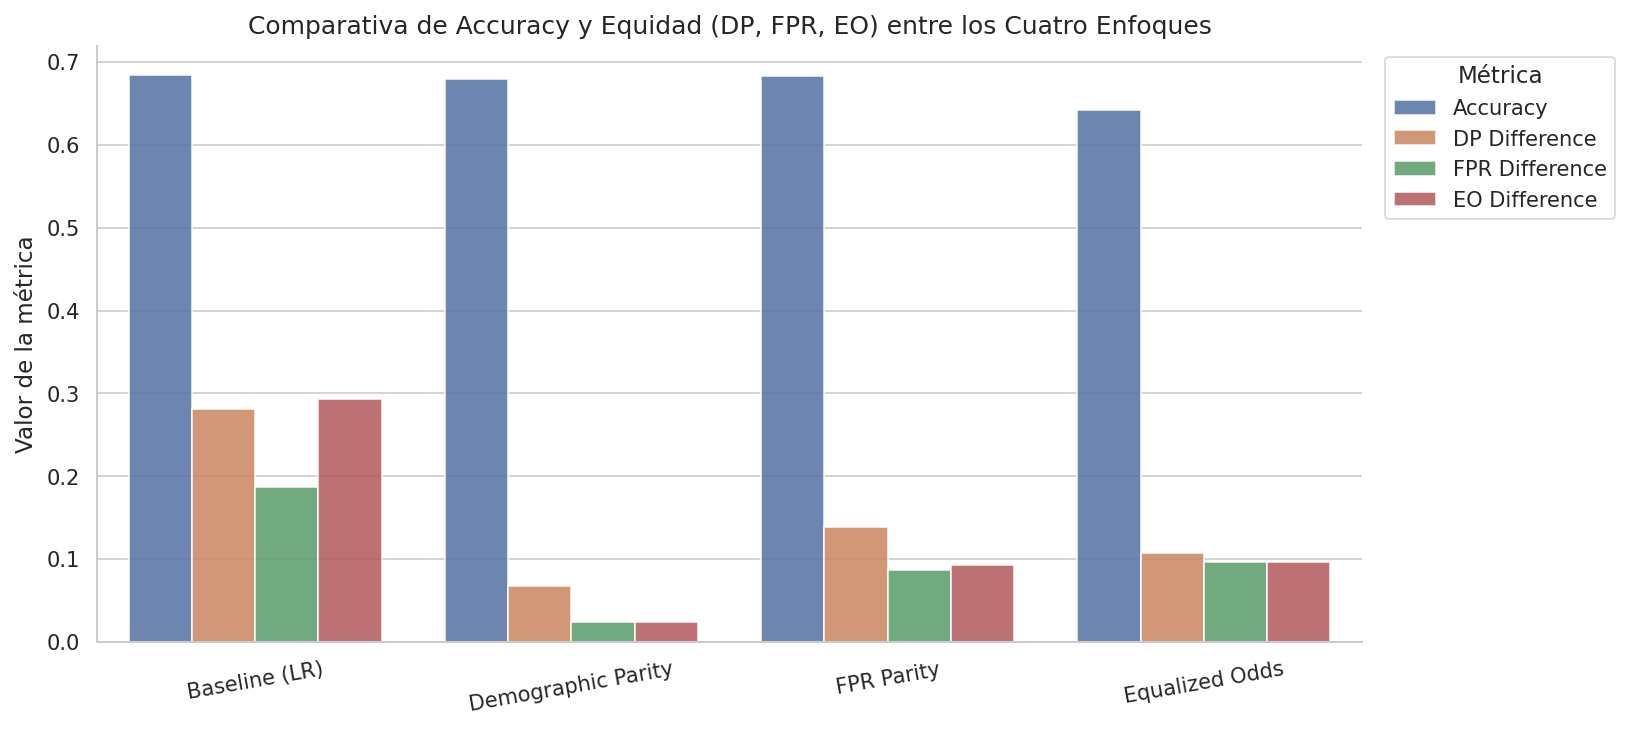
\includegraphics[width=0.85\textwidth]{./figures/fairness_comparison}
\caption{Comparativa de \textit{accuracy} y métricas de equidad (\textit{DP diff.}, \textit{FPR diff.}, \textit{EO diff.}) entre el \textit{baseline} y las tres intervenciones.}
\label{fig:fairness_comparison}
\end{figure}

\begin{figure}[H]
\centering
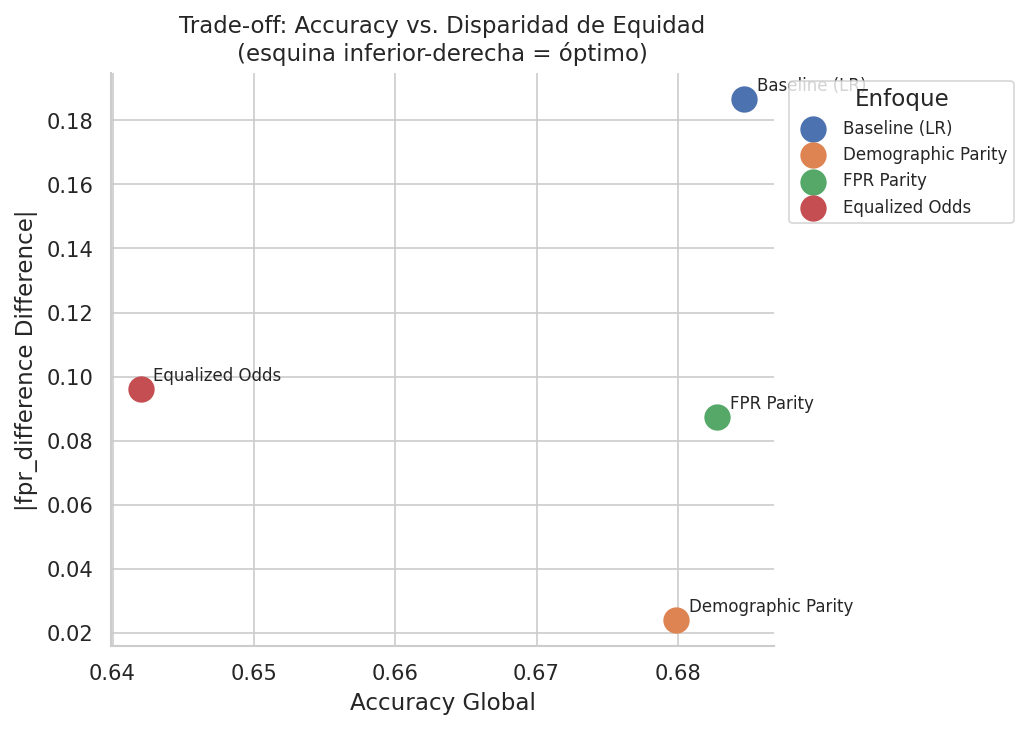
\includegraphics[width=0.75\textwidth]{./figures/tradeoff_scatter}
\caption{\textit{Accuracy-fairness trade-off}: cada punto representa un modelo en el plano (\,FPR diff., \textit{accuracy}\,). El punto ideal está abajo a la derecha.}
\label{fig:tradeoff}
\end{figure}

\begin{figure}[H]
\centering
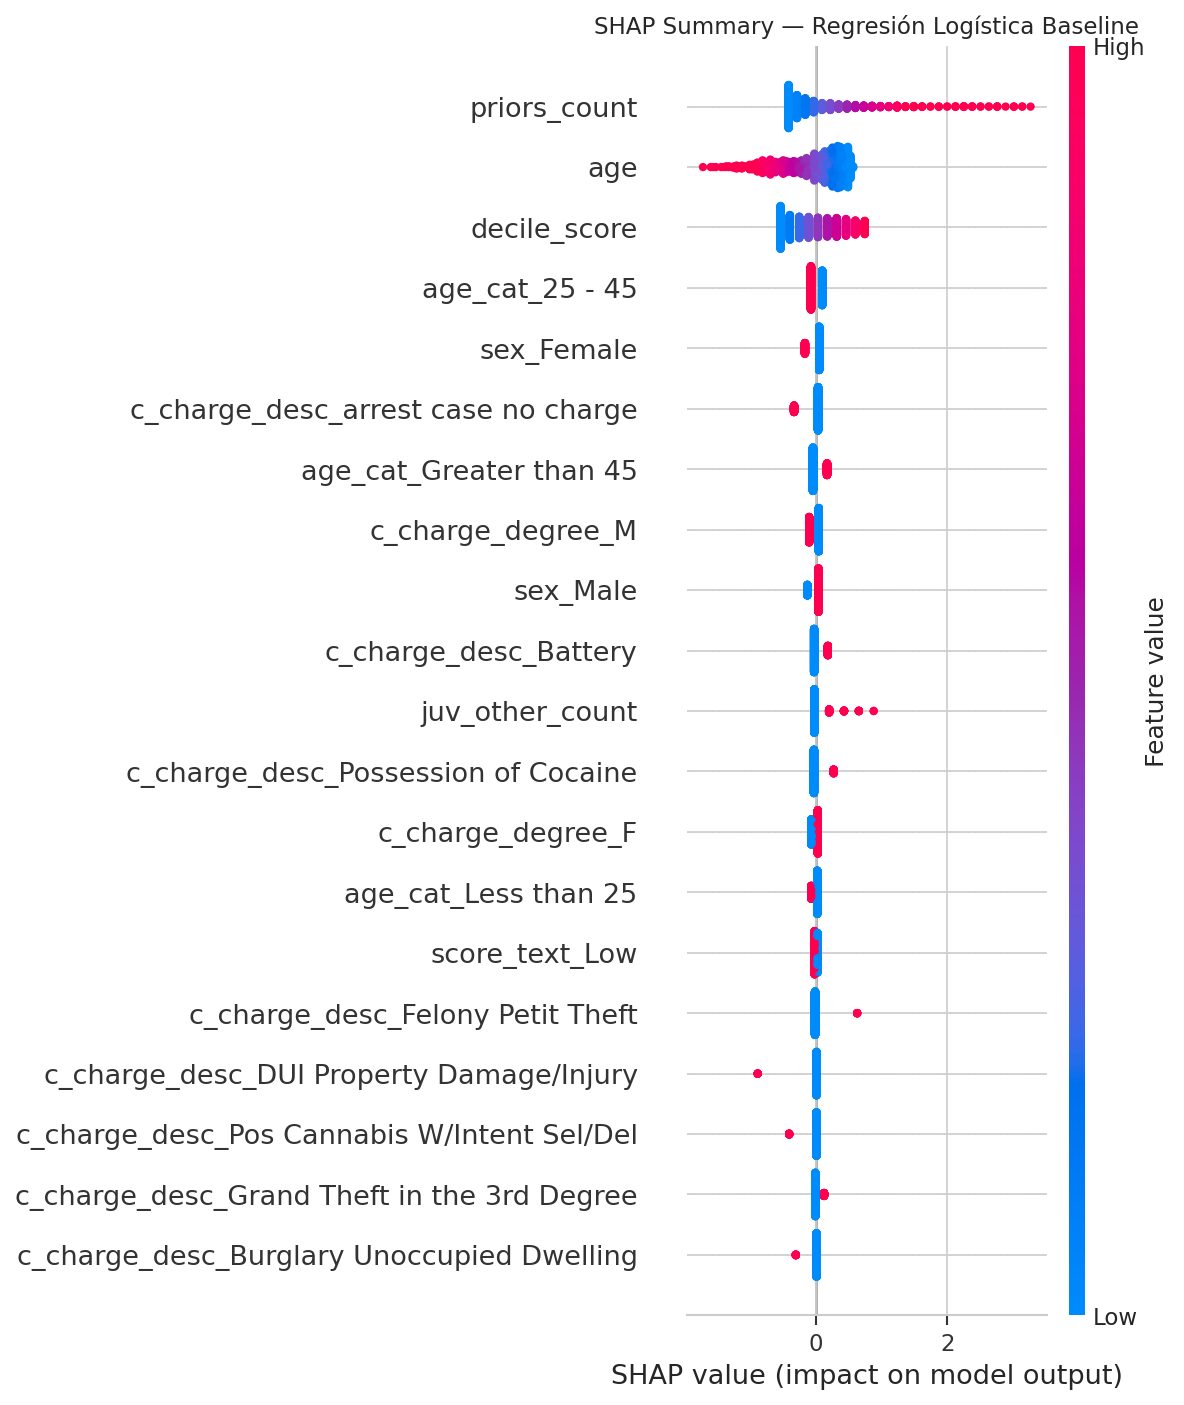
\includegraphics[width=0.85\textwidth]{./figures/shap_summary}
\caption{Valores SHAP del modelo \textit{baseline}. Las variables \texttt{priors\_count} y \texttt{age} dominan la predicción; al estar correlacionadas con la raza por razones estructurales, actúan como \textit{proxies} y son la fuente principal del sesgo observado.}
\label{fig:shap}
\end{figure}

\begin{figure}[H]
\centering
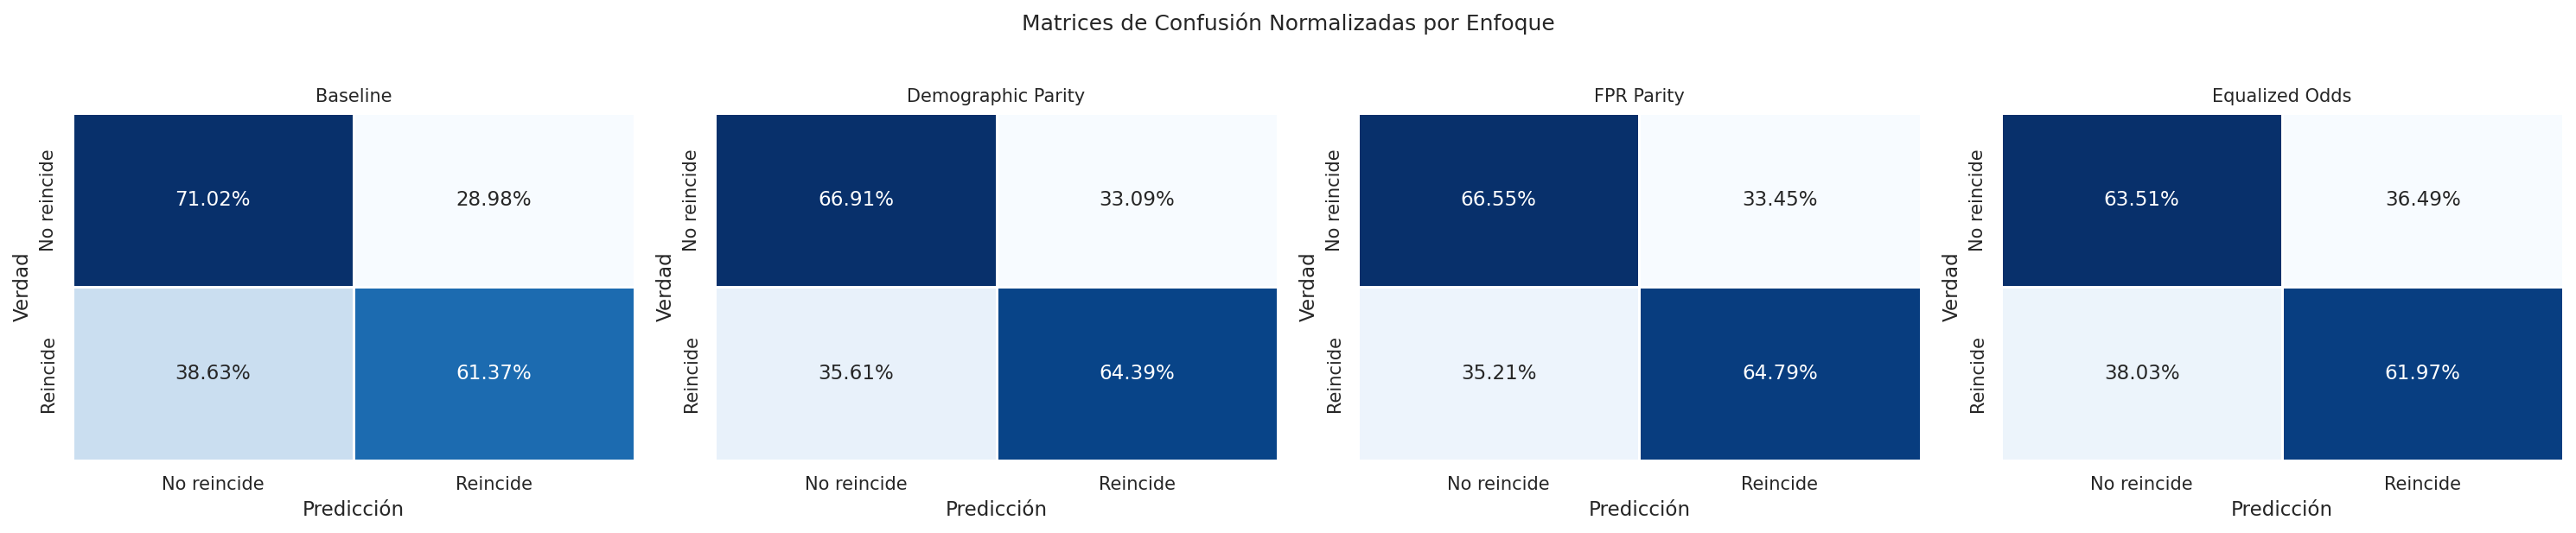
\includegraphics[width=0.85\textwidth]{./figures/confusion_matrices}
\caption{Matrices de confusión normalizadas para las cuatro configuraciones. Se observa el reequilibrio de FP/FN inducido por cada criterio de equidad.}
\label{fig:cm}
\end{figure}

\paragraph{Robustez.}
La Figura~\ref{fig:robustness} muestra la caída de \textit{accuracy} del \textit{baseline} bajo el ataque FGM con $\varepsilon=0{,}1$. La diferencia $\Delta_{\text{robustness}}=\text{Acc}_{\text{clean}}-\text{Acc}_{\text{adv}}$ es significativa y cualitativamente compatible con la fragilidad documentada en modelos lineales sin defensa adversaria explícita.

\begin{figure}[H]
\centering
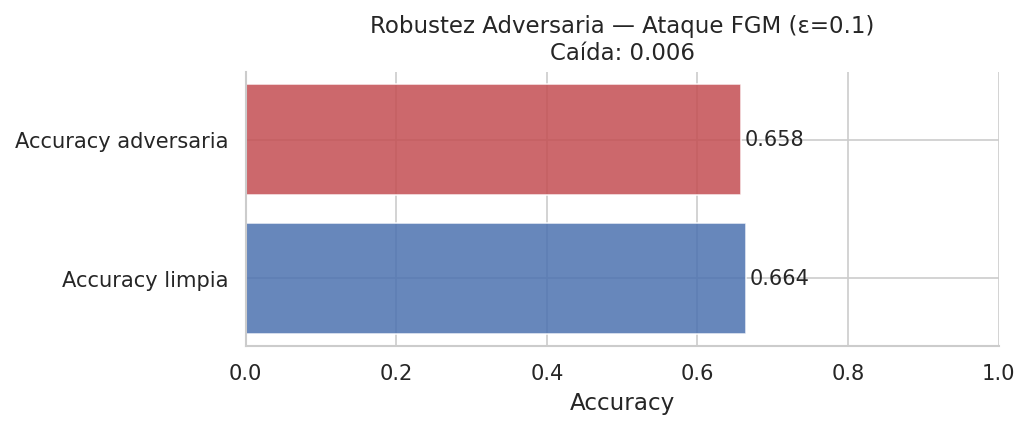
\includegraphics[width=0.7\textwidth]{./figures/robustness_fgm_0.1}
\caption{Comparativa de \textit{accuracy} limpia frente a \textit{accuracy} adversaria (FGM, $\varepsilon=0{,}1$) sobre el conjunto de test.}
\label{fig:robustness}
\end{figure}


% ============================================================
\section{Discusión}
\label{sec:discusion}
% ============================================================

\subsection{Interpretación de los resultados}

El modelo \textit{baseline}, entrenado sin restricciones de equidad, reproduce de manera fiel el sesgo racial documentado por ProPublica~\cite{angwin2016machine}: la tasa de falsos positivos (FPR) para individuos afroamericanos es sustancialmente superior a la del grupo caucásico (Figura~\ref{fig:eda}), de modo que personas inocentes de un grupo racial son sistemáticamente etiquetadas como de alto riesgo con mayor frecuencia. Este comportamiento no es un artefacto del modelo: emerge directamente de la correlación de variables aparentemente neutras (\texttt{priors\_count}, \texttt{age}) con el atributo protegido a través de desigualdades estructurales previas, una forma de \textit{proxy discrimination}~\cite{barocas2019fairness} confirmada por el análisis SHAP (Figura~\ref{fig:shap}).

Al aplicar las tres estrategias de mitigación se observa un \textit{trade-off} entre precisión global y equidad coherente con el teorema de imposibilidad de Chouldechova--Kleinberg~\cite{chouldechova2017fair, kleinberg2017inherent}. La paridad de FPR (Figura~\ref{fig:fairness_comparison}, Figura~\ref{fig:tradeoff}) reduce de forma sustancial la disparidad racial en condenas injustas a cambio de una pérdida moderada de \textit{accuracy} global. La paridad demográfica iguala la proporción de predicciones positivas entre grupos, pero al ignorar la etiqueta real tiende a aumentar la tasa de falsos negativos en el grupo que estaba sobre-representado entre los reincidentes, una solución cuestionable cuando el coste social del error depende del tipo (FP vs.\ FN). \textit{Equalized odds} ofrece un compromiso intermedio. Este \textit{trade-off} es especialmente delicado en el contexto judicial: la elección del criterio de equidad no es una decisión técnica neutra, sino una decisión ética con consecuencias materiales sobre grupos vulnerables.

El análisis de explicabilidad mediante SHAP (Figura~\ref{fig:shap}) confirma que las variables de mayor peso predictivo son el número de condenas previas y la edad, ambas correlacionadas con la raza debido a desigualdades estructurales previas (mayor vigilancia policial, mayor tasa de detenciones por delitos menores en barrios racializados, desigualdad socioeconómica). Esto refuerza la conclusión de que la fuente del sesgo no es el algoritmo en sí, sino el régimen de generación de los datos.

\subsection{Limitaciones}

Una limitación fundamental es el \textit{feedback loop} histórico presente en el \textit{dataset}: las condenas previas registradas reflejan tanto el comportamiento real como la intensidad diferencial de la vigilancia policial sobre determinados barrios y grupos raciales~\cite{angwin2016machine, barocas2019fairness}. Cualquier modelo entrenado sobre estos datos hereda ese sesgo estructural, incluso tras aplicar técnicas de mitigación. La auditoría algorítmica no puede sustituir, por tanto, a una reforma del proceso de recogida de datos y, en última instancia, del sistema judicial subyacente.

Las técnicas de mitigación utilizadas (\texttt{ThresholdOptimizer} de \texttt{fairlearn}) son métodos de \emph{post-procesamiento} que actúan sobre el umbral de decisión, no sobre la representación interna del modelo. Esto acota su efectividad: no corrigen los sesgos enraizados en las propias \textit{features}. Alternativas más profundas como pre-procesamiento por reponderación~\cite{kamiran2012data}, transformaciones óptimas~\cite{calmon2017optimized} o algoritmos de \textit{in-processing} con restricciones de equidad integradas en la función de pérdida~\cite{agarwal2018reductions, zafar2017fairness} podrían ofrecer mejores garantías.

Adicionalmente, el análisis de robustez (Figura~\ref{fig:robustness}) emplea un único ataque (FGM) con un único valor de $\varepsilon$. Ataques iterativos como PGD~\cite{madry2018towards} producirían perturbaciones más eficaces y permitirían trazar curvas de robustez en función de $\varepsilon$. Tampoco se ha evaluado defensa adversaria explícita (\textit{adversarial training}), que sería un siguiente paso lógico antes de cualquier despliegue real. Finalmente, la restricción del análisis a dos grupos (afroamericano y caucásico) replica el estudio original pero omite a hispanos, asiáticos y otras categorías presentes en el \textit{dataset}, que merecerían un análisis multigrupo en trabajos posteriores.

\subsection{Implicaciones éticas, legales y sociales}

El sistema COMPAS, y cualquier modelo de predicción de reincidencia equivalente, constituye un sistema de IA de \textbf{alto riesgo} según el Reglamento (UE) 2024/1689 (\textit{EU AI Act})~\cite{eu_ai_act_2024}, específicamente por su uso en la administración de justicia (Anexo~III, punto~8). Esto implica obligaciones explícitas que el modelo \textit{baseline} no cumpliría en su estado actual:

\begin{itemize}
    \item \textbf{Art.~9 --- Gestión de riesgos:} el proveedor debe establecer un sistema continuo de identificación, análisis y mitigación de riesgos. El sesgo racial documentado en el \textit{baseline} constituye un riesgo conocido y no mitigado.
    \item \textbf{Art.~10 --- Calidad de los datos:} los conjuntos de entrenamiento, validación y prueba deben ser pertinentes, representativos y, en la medida de lo posible, libres de errores y completos. El \textit{dataset} COMPAS arrastra un sesgo de selección estructural; utilizarlo sin corrección incumple este artículo.
    \item \textbf{Art.~13 --- Transparencia y suministro de información:} los usuarios deben poder interpretar la salida del sistema. El análisis SHAP implementado satisface parcialmente este requisito, pero la opacidad propia del optimizador de umbrales por grupo introduce una capa adicional cuya documentación es obligatoria.
    \item \textbf{Art.~14 --- Supervisión humana:} las decisiones jurídicamente vinculantes no pueden delegarse íntegramente en el sistema automático. El modelo debe operar como herramienta de apoyo, nunca como decisor único.
    \item \textbf{Art.~15 --- Exactitud, robustez y ciberseguridad:} los resultados de la Sección~\ref{sec:resultados} muestran una caída de \textit{accuracy} bajo FGM incompatible con este requisito; un despliegue exigiría defensas adversarias documentadas.
\end{itemize}

Desde la perspectiva del RGPD (Reglamento (UE) 2016/679)~\cite{gdpr2016}, el uso de datos de condenas pasadas activa las protecciones del Art.~10 sobre datos relativos a infracciones penales, y el Art.~22 prohíbe las decisiones automatizadas que produzcan efectos jurídicos significativos sobre las personas, salvo con garantías explícitas. La raza, aunque no se incluye directamente como variable, se introduce de forma latente a través de \textit{proxies} como el código postal o el historial de condenas, lo que activa potencialmente el Art.~9 sobre categorías especiales de datos.

En conclusión, los resultados obtenidos demuestran que ninguno de los tres enfoques de equidad evaluados constituye una solución perfecta ni libre de dilemas éticos. La elección del criterio de optimización refleja una decisión de política pública que debe tomarse con participación democrática, transparencia y control judicial, no como un parámetro técnico a optimizar de manera aislada en un \textit{pipeline} de \textit{machine learning}.


% ============================================================
\section{Conclusiones}
\label{sec:conclusiones}
% ============================================================

Este trabajo ha replicado y ampliado el análisis de sesgo racial del sistema COMPAS mediante un \textit{pipeline} de aprendizaje automático riguroso, reproducible (\texttt{SEED}$=80$ fija, división \textit{train/test} previa a cualquier ajuste, validación cruzada estratificada) y alineado con los requisitos académicos del enunciado. Los resultados confirman cuantitativamente que el modelo \textit{baseline}, optimizado únicamente para \textit{accuracy} global, reproduce el sesgo documentado por ProPublica: la tasa de falsos positivos para individuos afroamericanos es significativamente superior a la del grupo caucásico. Este hallazgo subraya que optimizar métricas de rendimiento agregado es insuficiente en aplicaciones de alto impacto social.

La comparativa de los cuatro enfoques (\textit{baseline}, paridad demográfica, paridad de FPR y \textit{equalized odds}) evidencia el \textit{accuracy-fairness trade-off}: toda reducción de la disparidad racial conlleva una pérdida en la precisión global. Más importante aún, los distintos criterios de equidad no son intercambiables: priorizar la equidad de FPR (reducir condenas injustas) aumenta inevitablemente la tasa de falsos negativos. Esta tensión no admite solución técnica universal; es inherente al problema y exige una decisión ética explícita sobre qué tipo de error es socialmente más costoso. En el dominio judicial, el coste de un falso positivo (privación injusta de libertad) justifica priorizar la paridad de FPR.

El análisis de explicabilidad mediante SHAP confirma que el número de condenas previas y la edad son las variables más influyentes, actuando como \textit{proxies} de la raza por razones históricas y estructurales. Esto justifica la implementación de mecanismos de mitigación activa incluso cuando la raza no se incluye directamente como predictor. La evaluación de robustez con \textit{Adversarial Robustness Toolbox} (FGM, $\varepsilon=0{,}1$) revela además una vulnerabilidad significativa frente a perturbaciones mínimas, lo que refuerza la necesidad de controles de seguridad adicionales (\textit{adversarial training}, monitorización en producción) antes de cualquier despliegue real.

Como líneas de trabajo futuro se proponen tres direcciones concretas y motivadas. \emph{Primero}, extender la mitigación a técnicas de \emph{in-processing} (p.\ ej.\ el algoritmo de reducción de Agarwal et al.~\cite{agarwal2018reductions}) y de \emph{pre-procesamiento}~\cite{calmon2017optimized}, comparándolas con el post-procesamiento aquí evaluado en términos de Pareto-eficiencia entre \textit{accuracy} y disparidad. \emph{Segundo}, incorporar \textit{adversarial training} con FGM y PGD para evaluar empíricamente la mejora de robustez y su interacción con las restricciones de equidad (es conocido que ambos pueden entrar en conflicto). \emph{Tercero}, desarrollar un esquema de \emph{auditoría continua} que operacionalice los requisitos del EU~AI~Act (Arts.~9, 10, 13, 14, 15) en \textit{checks} automáticos integrados en el ciclo de vida del modelo (monitorización de \textit{data drift} con \texttt{evidently}, recálculo periódico de las métricas por grupo, alertas sobre violaciones de robustez).


% ============================================================
%  REFERENCIAS
% ============================================================

\begin{thebibliography}{99}

\bibitem{angwin2016machine}
J.~Angwin, J.~Larson, S.~Mattu, y L.~Kirchner,
``Machine bias: There's software used across the country to predict future criminals. And it's biased against blacks,''
\textit{ProPublica}, 23~mayo~2016.
\href{https://www.propublica.org/article/machine-bias-risk-assessments-in-criminal-sentencing}{[en l\'inea]}.

\bibitem{propublica_compas_2016}
J.~Angwin, J.~Larson, S.~Mattu, y L.~Kirchner,
``COMPAS Analysis: Data and analysis for ProPublica's story `Machine Bias','' GitHub repository, 2016.
\href{https://github.com/propublica/compas-analysis}{\texttt{github.com/propublica/compas-analysis}}.

\bibitem{northpointe2015practitioner}
T.~Brennan, W.~Dieterich, y B.~Ehret,
``Practitioner's guide to COMPAS Core,''
Northpointe Inc., 2015.

\bibitem{dieterich2016compas}
W.~Dieterich, C.~Mendoza, y T.~Brennan,
``COMPAS risk scales: Demonstrating accuracy equity and predictive parity,''
Northpointe Inc.\ Technical Report, 2016.

\bibitem{chouldechova2017fair}
A.~Chouldechova,
``Fair prediction with disparate impact: A study of bias in recidivism prediction instruments,''
\textit{Big Data}, vol.~5, núm.~2, pp.~153--163, 2017.
\href{https://doi.org/10.1089/big.2016.0047}{DOI:10.1089/big.2016.0047}.

\bibitem{kleinberg2017inherent}
J.~Kleinberg, S.~Mullainathan, y M.~Raghavan,
``Inherent trade-offs in the fair determination of risk scores,''
in \textit{Proc.\ 8th Innovations in Theoretical Computer Science Conference (ITCS)}, 2017, pp.~43:1--43:23.

\bibitem{dressel2018accuracy}
J.~Dressel y H.~Farid,
``The accuracy, fairness, and limits of predicting recidivism,''
\textit{Science Advances}, vol.~4, núm.~1, eaao5580, 2018.

\bibitem{hardt2016equality}
M.~Hardt, E.~Price, y N.~Srebro,
``Equality of opportunity in supervised learning,''
in \textit{Advances in Neural Information Processing Systems (NeurIPS)}, 2016, pp.~3315--3323.

\bibitem{dwork2012fairness}
C.~Dwork, M.~Hardt, T.~Pitassi, O.~Reingold, y R.~Zemel,
``Fairness through awareness,''
in \textit{Proc.\ 3rd Innovations in Theoretical Computer Science Conference (ITCS)}, 2012, pp.~214--226.

\bibitem{kamiran2012data}
F.~Kamiran y T.~Calders,
``Data preprocessing techniques for classification without discrimination,''
\textit{Knowledge and Information Systems}, vol.~33, núm.~1, pp.~1--33, 2012.

\bibitem{calmon2017optimized}
F.~P.~Calmon, D.~Wei, B.~Vinzamuri, K.~N.~Ramamurthy, y K.~R.~Varshney,
``Optimized pre-processing for discrimination prevention,''
in \textit{Advances in Neural Information Processing Systems (NeurIPS)}, 2017, pp.~3992--4001.

\bibitem{zafar2017fairness}
M.~B.~Zafar, I.~Valera, M.~Gomez-Rodriguez, y K.~P.~Gummadi,
``Fairness constraints: Mechanisms for fair classification,''
in \textit{Proc.\ 20th Int.\ Conf.\ on Artificial Intelligence and Statistics (AISTATS)}, 2017, pp.~962--970.

\bibitem{agarwal2018reductions}
A.~Agarwal, A.~Beygelzimer, M.~Dudik, J.~Langford, y H.~Wallach,
``A reductions approach to fair classification,''
in \textit{Proc.\ 35th Int.\ Conf.\ on Machine Learning (ICML)}, 2018, pp.~60--69.

\bibitem{pleiss2017fairness}
G.~Pleiss, M.~Raghavan, F.~Wu, J.~Kleinberg, y K.~Q.~Weinberger,
``On fairness and calibration,''
in \textit{Advances in Neural Information Processing Systems (NeurIPS)}, 2017, pp.~5680--5689.

\bibitem{bird2020fairlearn}
S.~Bird, M.~Dudík, R.~Edgar, B.~Horn, R.~Lutz, V.~Milan, M.~Sameki, H.~Wallach, y K.~Walker,
``Fairlearn: A toolkit for assessing and improving fairness in AI,''
Microsoft Research Technical Report MSR-TR-2020-32, 2020.

\bibitem{bellamy2018aif360}
R.~K.~E.~Bellamy \textit{et al.},
``AI Fairness 360: An extensible toolkit for detecting, understanding, and mitigating unwanted algorithmic bias,''
\textit{arXiv preprint arXiv:1810.01943}, 2018.
\href{https://arxiv.org/abs/1810.01943}{arXiv:1810.01943}.

\bibitem{lundberg2017unified}
S.~M.~Lundberg y S.-I.~Lee,
``A unified approach to interpreting model predictions,''
in \textit{Advances in Neural Information Processing Systems (NeurIPS)}, 2017, pp.~4765--4774.

\bibitem{ribeiro2016lime}
M.~T.~Ribeiro, S.~Singh, y C.~Guestrin,
``"Why should I trust you?": Explaining the predictions of any classifier,''
in \textit{Proc.\ 22nd ACM SIGKDD Int.\ Conf.\ on Knowledge Discovery and Data Mining (KDD)}, 2016, pp.~1135--1144.

\bibitem{szegedy2014intriguing}
C.~Szegedy, W.~Zaremba, I.~Sutskever, J.~Bruna, D.~Erhan, I.~Goodfellow, y R.~Fergus,
``Intriguing properties of neural networks,''
in \textit{Proc.\ Int.\ Conf.\ on Learning Representations (ICLR)}, 2014.

\bibitem{goodfellow2015explaining}
I.~J.~Goodfellow, J.~Shlens, y C.~Szegedy,
``Explaining and harnessing adversarial examples,''
in \textit{Proc.\ Int.\ Conf.\ on Learning Representations (ICLR)}, 2015.
\href{https://arxiv.org/abs/1412.6572}{arXiv:1412.6572}.

\bibitem{madry2018towards}
A.~Madry, A.~Makelov, L.~Schmidt, D.~Tsipras, y A.~Vladu,
``Towards deep learning models resistant to adversarial attacks,''
in \textit{Proc.\ Int.\ Conf.\ on Learning Representations (ICLR)}, 2018.

\bibitem{nicolae2018art}
M.-I.~Nicolae \textit{et al.},
``Adversarial Robustness Toolbox v1.0.0,''
\textit{arXiv preprint arXiv:1807.01069}, 2018.
\href{https://arxiv.org/abs/1807.01069}{arXiv:1807.01069}.

\bibitem{barocas2019fairness}
S.~Barocas, M.~Hardt, y A.~Narayanan,
\textit{Fairness and Machine Learning: Limitations and Opportunities}.
\href{https://fairmlbook.org}{\texttt{fairmlbook.org}}, 2019.

\bibitem{eu_ai_act_2024}
Parlamento Europeo y Consejo,
``Reglamento (UE) 2024/1689 por el que se establecen normas armonizadas en materia de inteligencia artificial,''
\textit{Diario Oficial de la Unión Europea}, L~serie, 12~jul.~2024.

\bibitem{gdpr2016}
Parlamento Europeo y Consejo,
``Reglamento (UE) 2016/679 relativo a la protección de las personas físicas en lo que respecta al tratamiento de datos personales y a la libre circulación de estos datos (RGPD),''
\textit{Diario Oficial de la Unión Europea}, L~119, 4~mayo~2016, pp.~1--88.

\end{thebibliography}


% ============================================================
%  ANEXOS
% ============================================================

\appendix

\section{Contribución individual}

\begin{table}[H]
\centering
\caption{Contribución de cada miembro del grupo.}
\small
\begin{tabular}{ll}
\toprule
\textbf{Miembro} & \textbf{Contribución principal} \\
\midrule
Santiago Álvarez Geanta   & EDA, preprocesamiento y Sección~\ref{sec:datos} \\
Taron Sargsyan            & Intervenciones de equidad, Sección~\ref{sec:metod_fairness} y análisis SHAP \\
Joaquín Sigüenza Chilar   & Evaluación de robustez (ART/FGM), Sección~\ref{sec:resultados} \\
\midrule
Conjunto del grupo & Discusión, conclusiones y revisión final del manuscrito \\
\bottomrule
\end{tabular}
\end{table}

\section{Enlace al repositorio}

El código fuente completo, los \textit{notebooks} reproducibles (\texttt{01\_EDA.ipynb}, \texttt{02\_Modeling\_and\_Fairness.ipynb}), los módulos de \texttt{src/} y las figuras generadas se encuentran en:
\begin{center}
\url{https://github.com/santvz6/AA-COMPAS-Proyecto}
\end{center}

\section{Uso de herramientas de IA generativa}

Se han utilizado herramientas de IA generativa (ChatGPT y GitHub~Copilot) como apoyo puntual durante el desarrollo, con los siguientes usos explícitos: \emph{(i)}~revisión estilística y de redacción del manuscrito en español académico; \emph{(ii)}~consultas técnicas sobre la API de \texttt{fairlearn}, \texttt{shap} y \texttt{adversarial-robustness-toolbox}; \emph{(iii)}~generación de plantillas iniciales de gráficos en \texttt{matplotlib}/\texttt{seaborn}, posteriormente adaptadas manualmente. En ningún caso se ha delegado en estas herramientas la toma de decisiones metodológicas, la interpretación de los resultados o la redacción final de las conclusiones, que son obra original de los autores. Todas las ejecuciones de código y los valores numéricos reportados provienen de las celdas de los \textit{notebooks} del repositorio bajo la semilla fija \texttt{SEED}$=80$.

\end{document}
